During our analysis described in \Cref{sub:publication-analysis}, it was
impossible to locate any relevant works that could address the second research
question (RQ2). As a result, it will be necessary to tackle this question and
strive to answer it.

As of the time of writing this paper, the design of the proposed tool is not
yet finalised. We have only developed initial ideas about how we will approach
the problem and have created a sketch of the proposed tool architecture, which
is shown in \Cref{fig:tool-architecture}.

\begin{figure*}[!htb]
  \caption{Candidate tool architecture}
  \label{fig:tool-architecture}
  \centering
  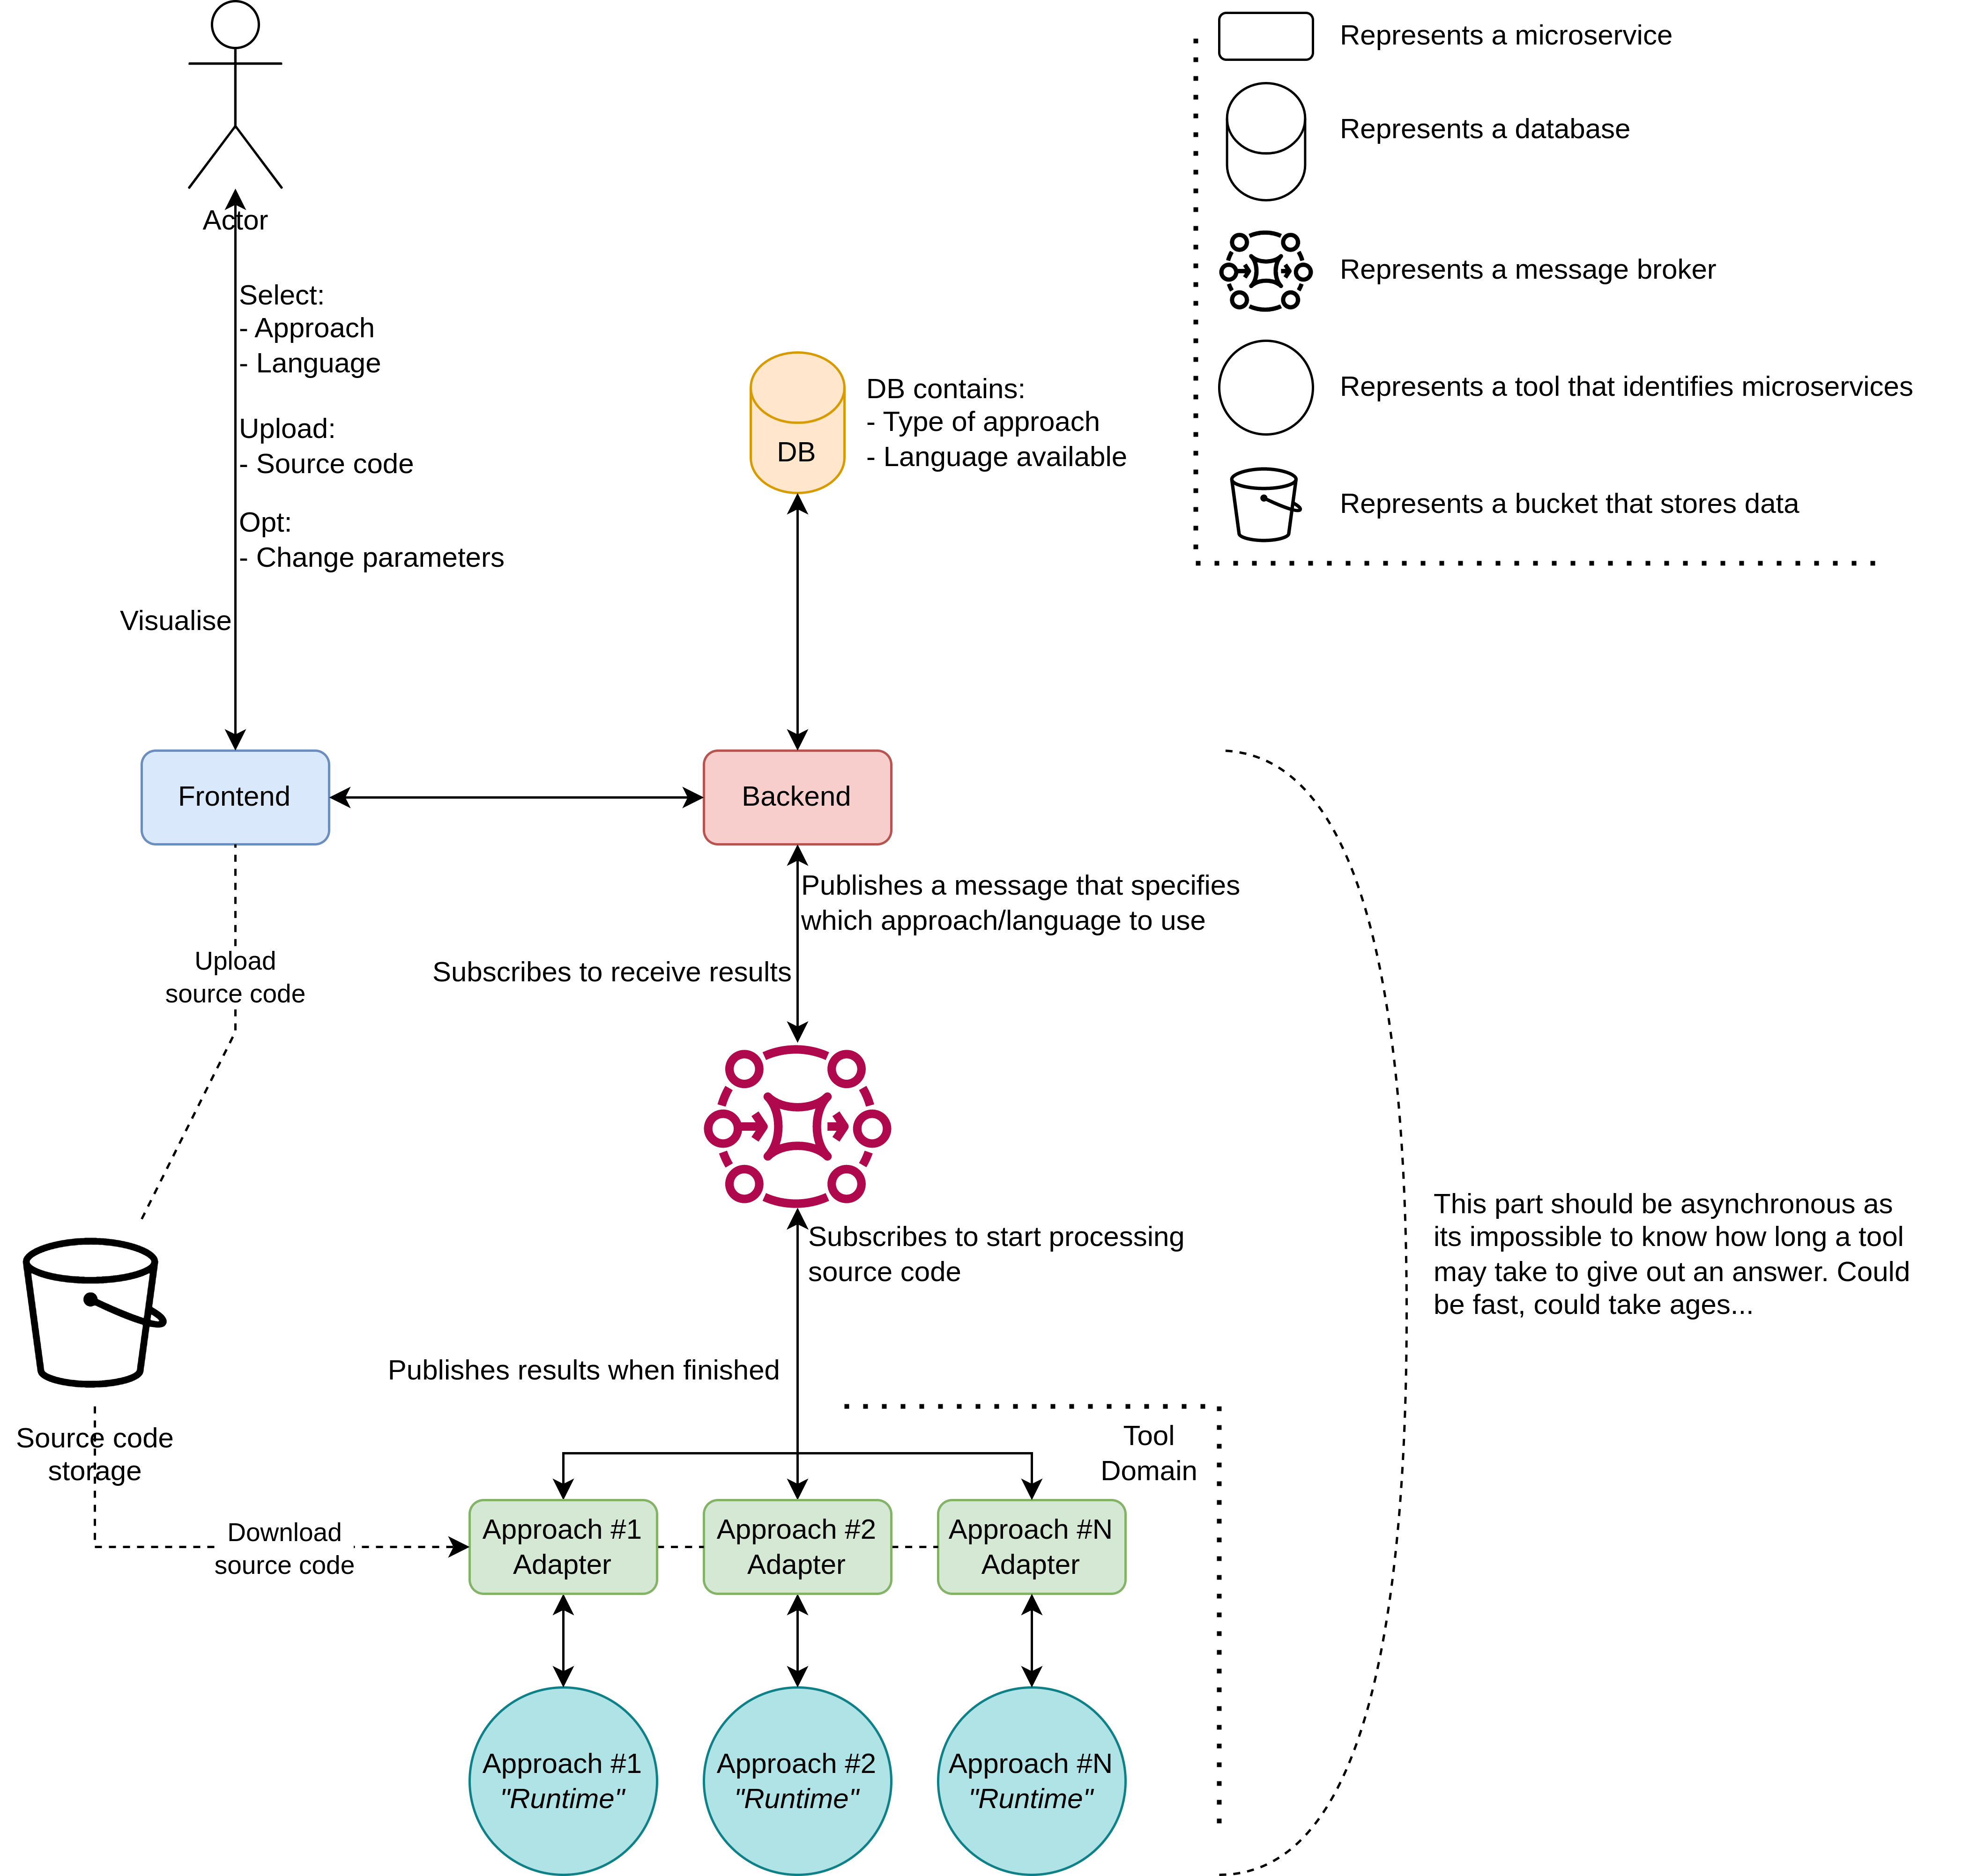
\includegraphics[width=\textwidth]{thesis-architecture.drawio}
\end{figure*}

The proposed tool architecture consists of three distinct components. The
frontend is responsible for the interface between the tool logic and the user.
The tool domain contains adapters for each individual tool and the tool
runtime, which receives the monolithic input and generates the candidate
microservices. The backend serves as a bridge between the frontend, the
database of available tools, and the tool domain.

The main role of the backend component in the proposed tool architecture is to
initiate jobs and notify the frontend when a given job has been completed. A
job consists of the process of identifying microservices from a given
monolithic input, which is then completed when the output containing the
identified microservices is produced. To avoid potential bottlenecks when
multiple jobs are run concurrently, the backend does not perform these tasks
directly but rather delegates them to the individual tools, therefore acting
like a bridge.

In the tool domain, the purpose of the adapter is to provide a consistent
interface for interacting with the tool runtime, regardless of the specific
input and output formats that it uses. This is important because different
tools may accept different inputs and produce different outputs, such as JSON
or raw code. By using an adapter to translate between these formats, it becomes
easier to process the inputs and outputs of the tool and integrate them with
the overall tool logic. The tool runtime receives the monolithic input and
generates the candidate microservices, while the adapter serves as a
``middleman'' between the tool runtime and the other components of the
architecture.

One of the first decisions that we have considered is which target platform the
tool should support. There are three major platforms that are relevant for this
purpose: macOS, Windows, and Linux. Determining which of these platforms to
focus on would require extensive surveying to ensure that the tool will be used
by the intended audience. While market share data suggests that Windows is the
most widely used desktop operating system, followed by macOS and Linux
\cite{desktop-usage-worldwide}, this may not necessarily reflect the operating
systems used by the architects, engineers, and developers who are responsible
for migration. Given the limited time frame, it is infeasible to conduct a
thorough survey to determine the preferred operating system of this target
audience. As a result, we have decided to adopt a more cross-platform solution.
After evaluating the options, we have determined that the browser is the most
suitable platform for this purpose.

Ideally, each component of the proposed tool architecture would be deployed as
a microservice in a Docker container to facilitate scalability and
cross-platform deployment. This is especially important for the tool runtime
component, as it is uncertain at this point whether the tools will take
advantage of multithreading. By using Docker, we can create a new container for
each job, which would allow us to handle multiple jobs concurrently and avoid
the need for users to wait for their jobs to complete. Of course, it is
possible that certain tool limitations may prevent us from implementing this
approach, but it is our goal to use microservices and Docker to the greatest
extent possible to ensure the flexibility and scalability of the tool.

Given that the tasks performed by the tool runtime component are asynchronous,
the communication between the tool runtime and the backend cannot be based on
synchronous HTTP request-response cycles. Instead, we will use a message queue
to connect the two components, with the use of message brokers. The backend
will send a message to initiate a job, which will be picked up by the
appropriate adapter and executed by the tool runtime. Once the job is
completed, the tool runtime will send another message to the backend to
indicate that it is finished. This approach allows us to process multiple jobs
concurrently and avoid potential bottlenecks in the communication between the
tool runtime and the backend.
